\chapter{A Cross-Vendor Firmware Footprint Analysis Tool}
\label{chap:footprint-tool}

\section*{Introduction}

Comparing STMicroelectronics against a competing vendor is, at bottom, a measurement
problem: the same workload is built for both platforms and the resulting binaries are
weighed against one another. One of the most revealing measurements is the
\emph{memory footprint} of the firmware --- how much flash and RAM a given software stack
consumes once compiled and linked. Footprint is easy to define but tedious to compare
fairly across ecosystems, because two vendors rarely name, split, or organise their code
the same way. To make this comparison reproducible rather than artisanal, we designed and
built a dedicated desktop and command-line application, \emph{MCU Workflow Studio}, that
ingests the linker output of two builds and produces a layer-aware, explainable footprint
comparison between an STM32 reference and a competitor.

This chapter documents that tool as an engineering contribution in its own right. We first
state the problem it solves and the requirements we set for it, then describe its
architecture and its end-to-end pipeline, the implementation choices behind its
deterministic core and its optional language-model assistance, how it plugs into the wider
benchmarking effort, and finally its concrete value and its current limitations.

\section{The cross-vendor footprint problem}
\label{sec:tool-problem}

The flash and RAM budget of a microcontroller unit (MCU) is a hard constraint. Every
kilobyte of code competes with application logic for a fixed amount of on-chip memory, and
it ripples into device cost, power, and the headroom left for future features. When we
benchmark a software stack --- a Universal Serial Bus (USB) device stack, a real-time
operating system integration, and so on --- the footprint each vendor charges for the same
functionality is
therefore a first-class metric.

Measuring it fairly is the difficult part. A modern build links application code against a
vendor software development kit (SDK) whose drivers, middleware, and startup code are structured to that
vendor's own conventions. The same peripheral initialisation appears as
\texttt{HAL\_GPIO\_Init} on STM32, as \texttt{GPIO\_PinInit} on one competitor, and as
\texttt{fsl\_gpio} routines on another; equivalent middleware sits in different modules, and
the boundary between "driver" and "system runtime" is drawn differently in each toolchain.
Doing the comparison by hand means reading two linker maps side by side, guessing which
symbol on one side corresponds to which on the other, and summing kilobytes into comparable
buckets --- slow, subjective, and impossible to reproduce exactly two weeks later.

We set the tool a small number of firm requirements. It had to be \textbf{deterministic and
reproducible}, so that the same inputs always yield the same verdict. It had to be
\textbf{layer-aware}, grouping symbols into architectural layers so that "ST spends more in
the hardware abstraction layer (HAL)" can be stated precisely. Its symbol matching had to be
\textbf{explainable}, attaching a confidence and a reason to every correspondence rather
than hiding behind a black box. It had to treat \textbf{ST as the reference} against which
each competitor is measured. And it had to \textbf{export} its results in formats the rest
of the report can consume directly.

\section{Design and architecture}
\label{sec:tool-architecture}

The tool is organised as a thin set of user interfaces wrapped around a deterministic
comparison core, with an SQLite-backed knowledge base alongside and an optional,
off-by-default block of language-model assistance. Figure~\ref{fig:tool-architecture}
shows the arrangement. Data flows top to bottom: a build's linker map enters through the
ingestion layer, is classified into architectural layers, is compared symbol by symbol in
the core, and leaves as a set of exported artefacts.

\begin{figure}[H]
\centering

\includegraphics[width=\textwidth]{Figures/footprint-tool/architecture.pdf}
\caption{Layered architecture of the footprint-analysis tool. A deterministic comparison
core (ingestion, classification, mapping, comparison, export) is wrapped by the user
interfaces and backed by an SQLite knowledge base; an optional, off-by-default
AI-assistance column refines the mapping without ever sitting on the critical path.}
\label{fig:tool-architecture}
\end{figure}

\begin{figure}[H]
\centering

\includegraphics[width=\textwidth]{Figures/footprint-tool/use-case.pdf}
\caption{UML use-case diagram of MCU Workflow Studio~v0.2.0. Five actors interact with
twenty use cases grouped by concern: the benchmark engineer drives the core analysis, the
technical reviewer validates low-confidence mappings, the CI/CD pipeline runs scripted
headless benchmarks, the LLM service (optional, dashed) enriches the mapping, and the
equivalence miner maintains the cross-vendor knowledge base.}
\label{fig:tool-use-case}
\end{figure}

\begin{figure}[H]
\centering

\includegraphics[width=\textwidth]{Figures/footprint-tool/sequence.pdf}
\caption{UML sequence diagram of a complete footprint benchmark run. The workflow service
orchestrates twelve steps: parsing both linker maps, classifying symbols into layers,
querying the equivalence database, scoring candidates with twelve weighted signals,
computing per-layer deltas, evaluating firmware quality metrics, and emitting the run
manifest alongside all export artefacts.}
\label{fig:tool-sequence}
\end{figure}

Two interfaces sit on top of the same engine: a desktop graphical user interface (GUI) built with PySide6
(the Qt binding for Python)~\cite{pyside6}, which provides over fourteen analysis tabs ---
including interactive charts, a mapping mind-map visualisation panel, a review queue, and a
project-scoped chat assistant --- and a command-line interface for scripted and reproducible
runs. Both call
into a single \emph{workflow service} that owns the data models and drives every stage.
Persistence is handled by SQLite~\cite{sqlite}: a vendor registry of aliases and naming
prefixes, a knowledge store of confirmed correspondences, an optional feedback store, and a
history of past runs. The block of language-model features on the right is genuinely
optional --- the deterministic path produces a complete result without it --- and we return
to it in Section~\ref{sec:tool-ai}. Table~\ref{tab:tool-io} lists what the tool consumes
and what it produces.

\begin{table}[H]
\centering
\caption{Principal inputs and outputs of the tool.}
\label{tab:tool-io}
\begin{tabularx}{\textwidth}{l X}
\toprule
\textbf{Inputs} & \textbf{Description} \\
\midrule
IAR EWARM \texttt{.map} ($\times 2$) & Linker maps of the source (STM32) and target (competitor) builds; the only required inputs. \\
Prior workbook (\texttt{.xlsx}) & Optional earlier results re-used as a baseline. \\
Vendor identifiers & Source and target vendor names (default \texttt{stm32}/\texttt{nxp}) that select the alias and prefix tables. \\
\midrule
\textbf{Outputs} & \textbf{Description} \\
\midrule
\texttt{benchmark\_results.xlsx} & Per-layer and global flash/RAM comparison with a verdict. \\
Scoped CSV/JSON/XLSX & Filtered exports for downstream processing. \\
Review queue (JSON/CSV) & Low-confidence mappings prioritised for manual confirmation. \\
Mapping diagnostics (JSON) & Per-pair signal breakdown and acceptance decisions. \\
GUI payload (JSON) & Pre-rendered data for the desktop interface. \\
PDF report (optional) & Eight-page narrative summary with charts, quality grade, and enhancement roadmap. \\
Run manifest (JSON) & Tool version, input checksums, equivalence DB hash, and deterministic mode for reproducibility. \\
\bottomrule
\end{tabularx}
\end{table}

\section{The benchmarking pipeline}
\label{sec:tool-pipeline}

A benchmark run is a fixed sequence of stages, sketched in
Figure~\ref{fig:tool-pipeline}. The solid path is purely deterministic; the dashed stages
are the optional language-model steps, which are disabled by default and can be switched on
without changing anything else. After validating its inputs, the tool parses both linker
maps into a common in-memory model --- build metadata, an overall footprint, and the list
of modules and functions with their code and data sizes. Each symbol is then classified
into an architectural layer, and the vendor knowledge (aliases, prefixes, prior matches) is
prepared.

The heart of the run is the mapping stage, where each STM32 symbol is matched to its
closest competitor counterpart by combining several similarity signals into a single,
explainable score. The accepted matches are then aggregated: the tool computes the flash
and RAM totals per layer and globally for both sides, compares them, and emits a verdict
together with recommendations and a root-cause breakdown of where the difference comes
from. Finally it persists the quality of the pair and composes its exports; the optional
advisor, PDF report, and run-history entry are produced only if requested.

\begin{figure}[H]
\centering
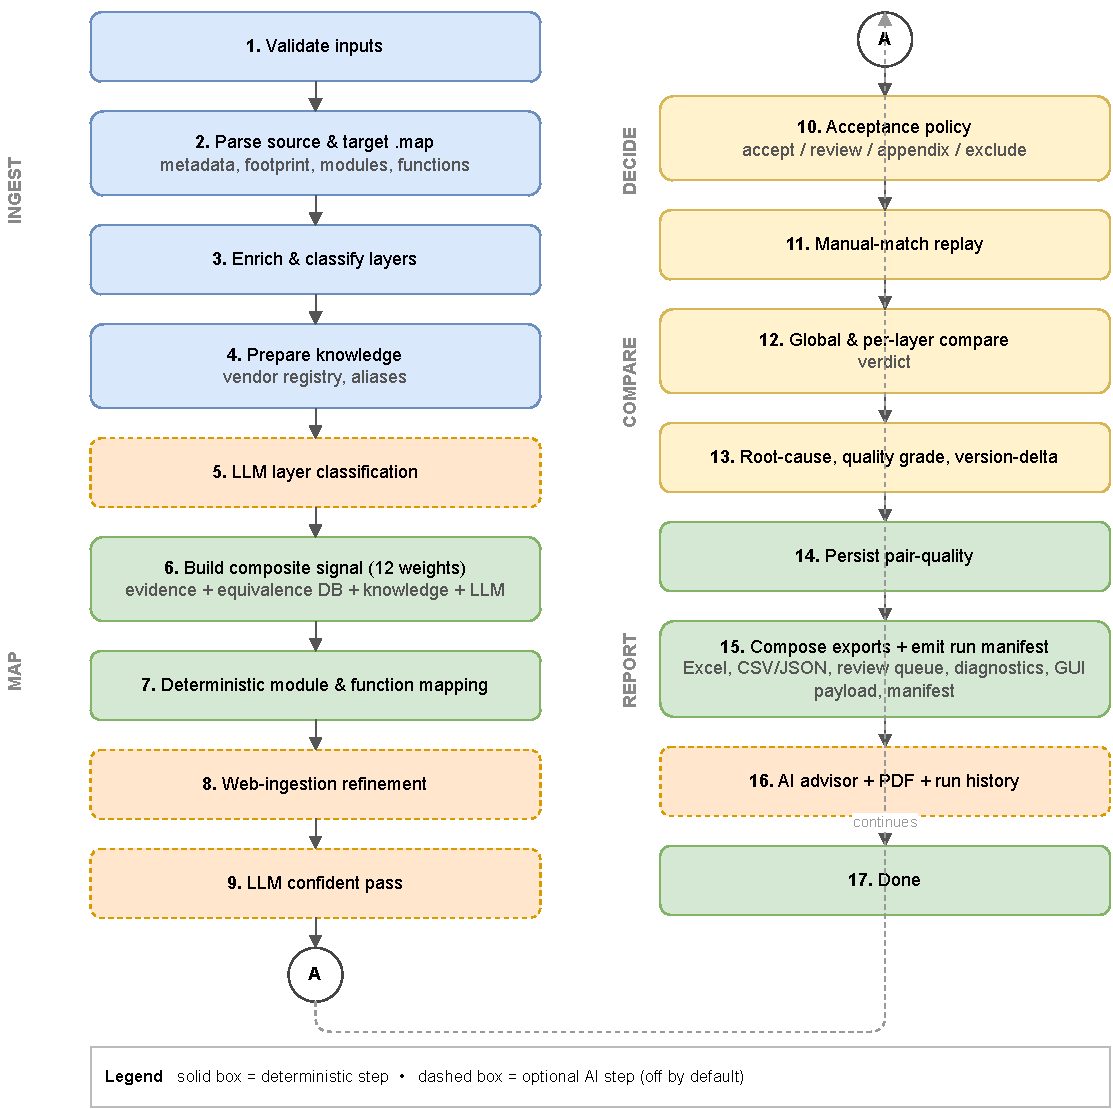
\includegraphics[width=0.9\textwidth]{Figures/footprint-tool/pipeline.pdf}
\caption{End-to-end benchmark pipeline, from linker-map ingestion to report generation.
Dashed stages are optional AI-assisted steps that are disabled by default; the solid
deterministic path runs end to end on its own.}
\label{fig:tool-pipeline}
\end{figure}

A second, lighter mode produces a single-map footprint summary --- validate, parse, classify,
and write a footprint workbook --- which is useful when only one build is available or to
sanity-check a map before a full comparison.

\section{Implementation}
\label{sec:tool-implementation}

The tool is written entirely in Python ($\geq$~3.11)~\cite{python}, with a small,
deliberately conventional dependency set summarised in Table~\ref{tab:tool-stack}. We
favoured the standard library wherever it was sufficient: all persistence uses the built-in
SQLite engine~\cite{sqlite}, and every network call to a language model goes through the
standard \texttt{urllib} module rather than a vendor SDK, which keeps the executable small
and the dependency surface auditable. The whole application can be packaged into a
stand-alone Windows executable with PyInstaller~\cite{pyinstaller}.

\begin{table}[H]
\centering
\caption{Implementation stack and the role of each external dependency.}
\label{tab:tool-stack}
\begin{tabularx}{\textwidth}{l l X}
\toprule
\textbf{Concern} & \textbf{Technology} & \textbf{Role in the tool} \\
\midrule
Language & Python $\geq$ 3.11 \cite{python} & Entire code base (version 0.2.0). \\
Desktop GUI & PySide6 / Qt \cite{pyside6} & 14+ tab windows, mind-map panel, chat assistant. \\
Tabular export & pandas \cite{pandas} & Scoped CSV/JSON/Excel export. \\
Excel I/O & openpyxl \cite{openpyxl} & Reads prior workbooks, writes results. \\
Charts \& PDF & matplotlib \cite{matplotlib} & Figures in the 8-page PDF report. \\
Persistence & SQLite \cite{sqlite} & Knowledge base, equivalence store, run history. \\
Packaging & PyInstaller \cite{pyinstaller} & Stand-alone Windows executable. \\
\bottomrule
\end{tabularx}
\end{table}

\subsection{Parsing linker maps and classifying layers}
\label{sec:tool-parsing}

The single required input is the linker map emitted by the IAR Embedded Workbench for ARM
(EWARM) toolchain~\cite{iar-ewarm}. The parser reads this map and reconstructs, for
each module and function, the read-only code and data it contributes and the read-write data
it reserves. From these we derive the two footprint figures the benchmark cares about: flash
occupancy as the sum of read-only code and read-only data, and RAM occupancy as the
read-write data. This is a \emph{static} measurement taken from the linked image; it captures
what the firmware costs to store, not its dynamic stack or heap behaviour at run time, and we
are careful to present it as such.

Each symbol is then assigned to one of four architectural layers --- application, middleware,
low-level driver, or system runtime --- by a deterministic classifier driven by module names,
known vendor prefixes, and section attributes. This layering is what lets the final report say
not merely that one firmware is larger, but \emph{where} it is larger, which is far more useful
when the goal is to understand a vendor's engineering trade-offs.
Figure~\ref{fig:tool-layer-classification} details the decision flow.

\begin{figure}[H]
\centering
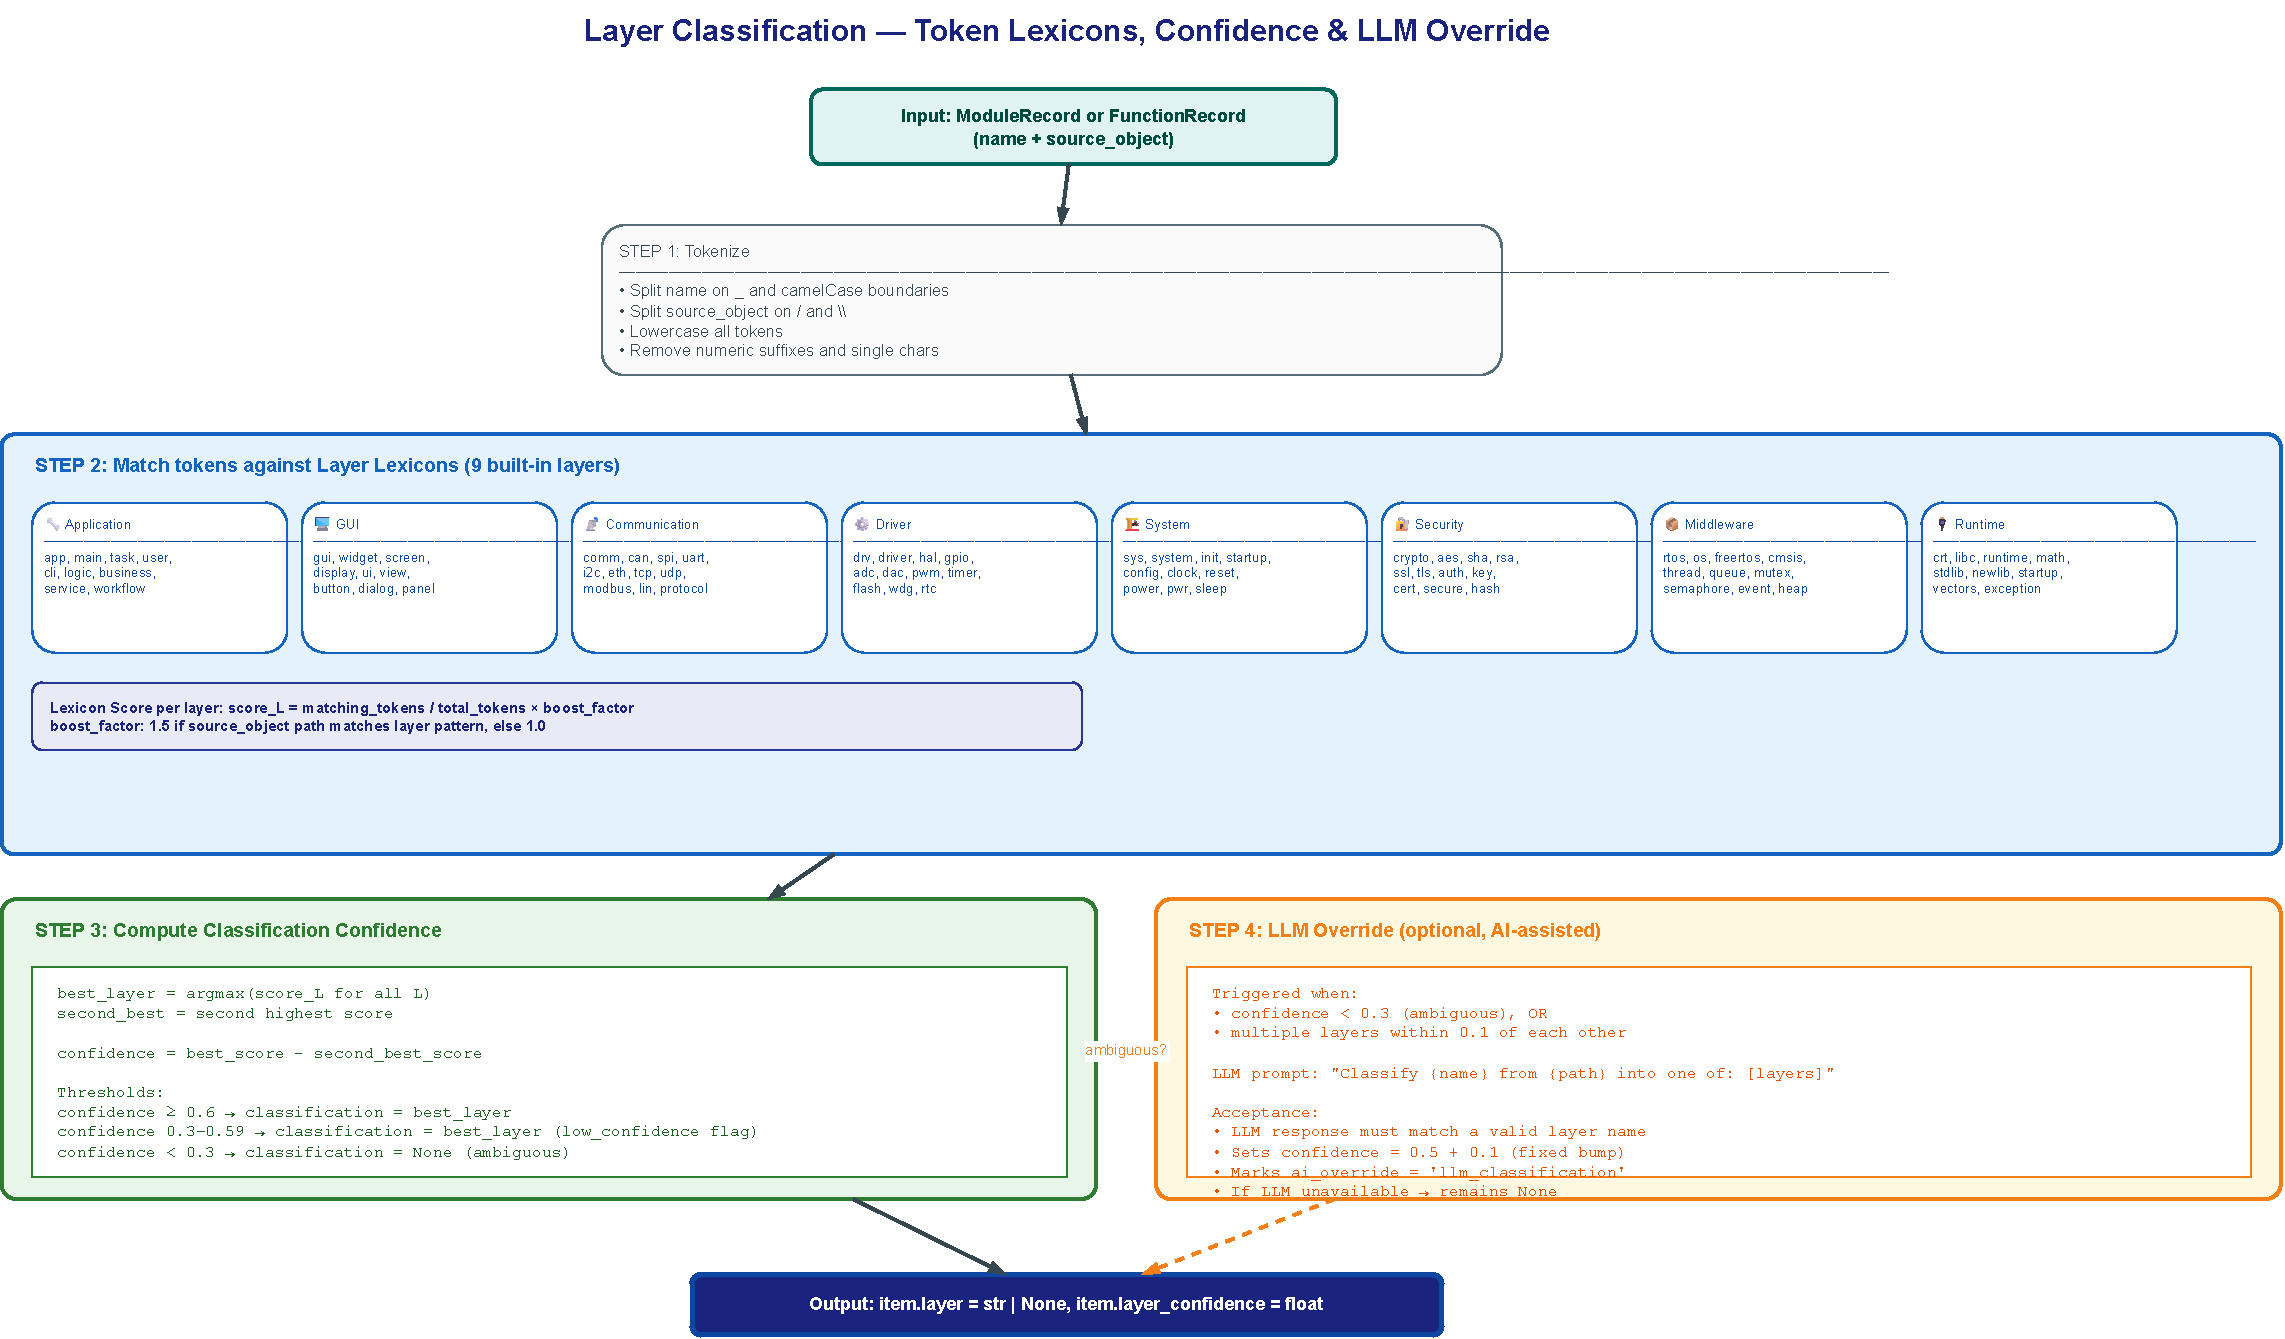
\includegraphics[width=\textwidth]{Figures/footprint-tool/layer-classification.pdf}
\caption{Layer-classification decision flow. Each symbol's tokens are matched against
priority-ordered lexicons (system, middleware, low-level, application); the first match
determines the layer with an associated confidence.}
\label{fig:tool-layer-classification}
\end{figure}

\subsection{The multi-signal mapping engine}
\label{sec:tool-mapping}

Matching ST symbols to their competitor counterparts is the part that, done manually, costs the
most time and is the least repeatable, so it received the most care. Rather than rely on name
similarity alone --- which fails precisely when two vendors name the same function differently
--- the engine scores each candidate pair by combining twelve weighted signals into a single,
explainable confidence value. Role similarity and alias similarity carry the most weight
(0.18 each), followed by name similarity and operation similarity (0.12 each), external
references and signature cues (0.10 each), footprint proximity (0.08), object similarity
(0.06), context cues (0.04), and three knowledge-base priors (history, board-pair,
scenario --- contributing the remaining 0.02). The weights sum to exactly~1.0.
Figure~\ref{fig:tool-weights} shows the relative weights, and
Figure~\ref{fig:tool-scoring-signals} expands the computation and penalty mechanics of each
signal.

\begin{figure}[H]
\centering
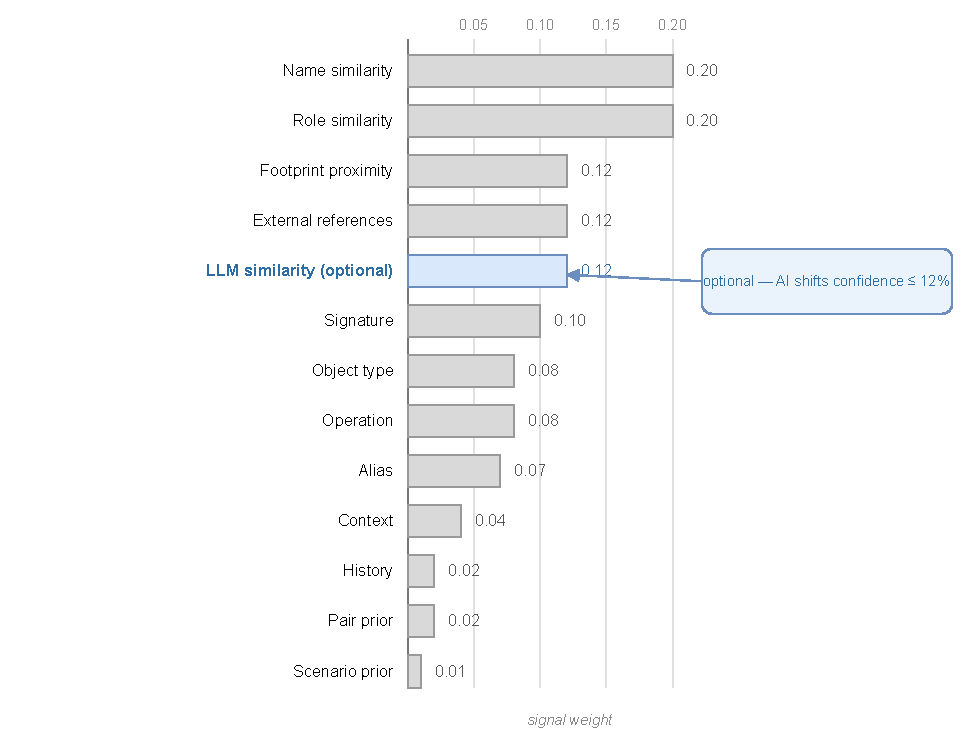
\includegraphics[width=0.88\textwidth]{Figures/footprint-tool/weights.pdf}
\caption{Relative weights of the signals combined by the deterministic mapping scorer. Name
and role similarity dominate; the optional LLM-similarity signal (highlighted) is capped so
that AI assistance can shift a candidate's confidence by at most twelve percent.}
\label{fig:tool-weights}
\end{figure}

\begin{figure}[H]
\centering
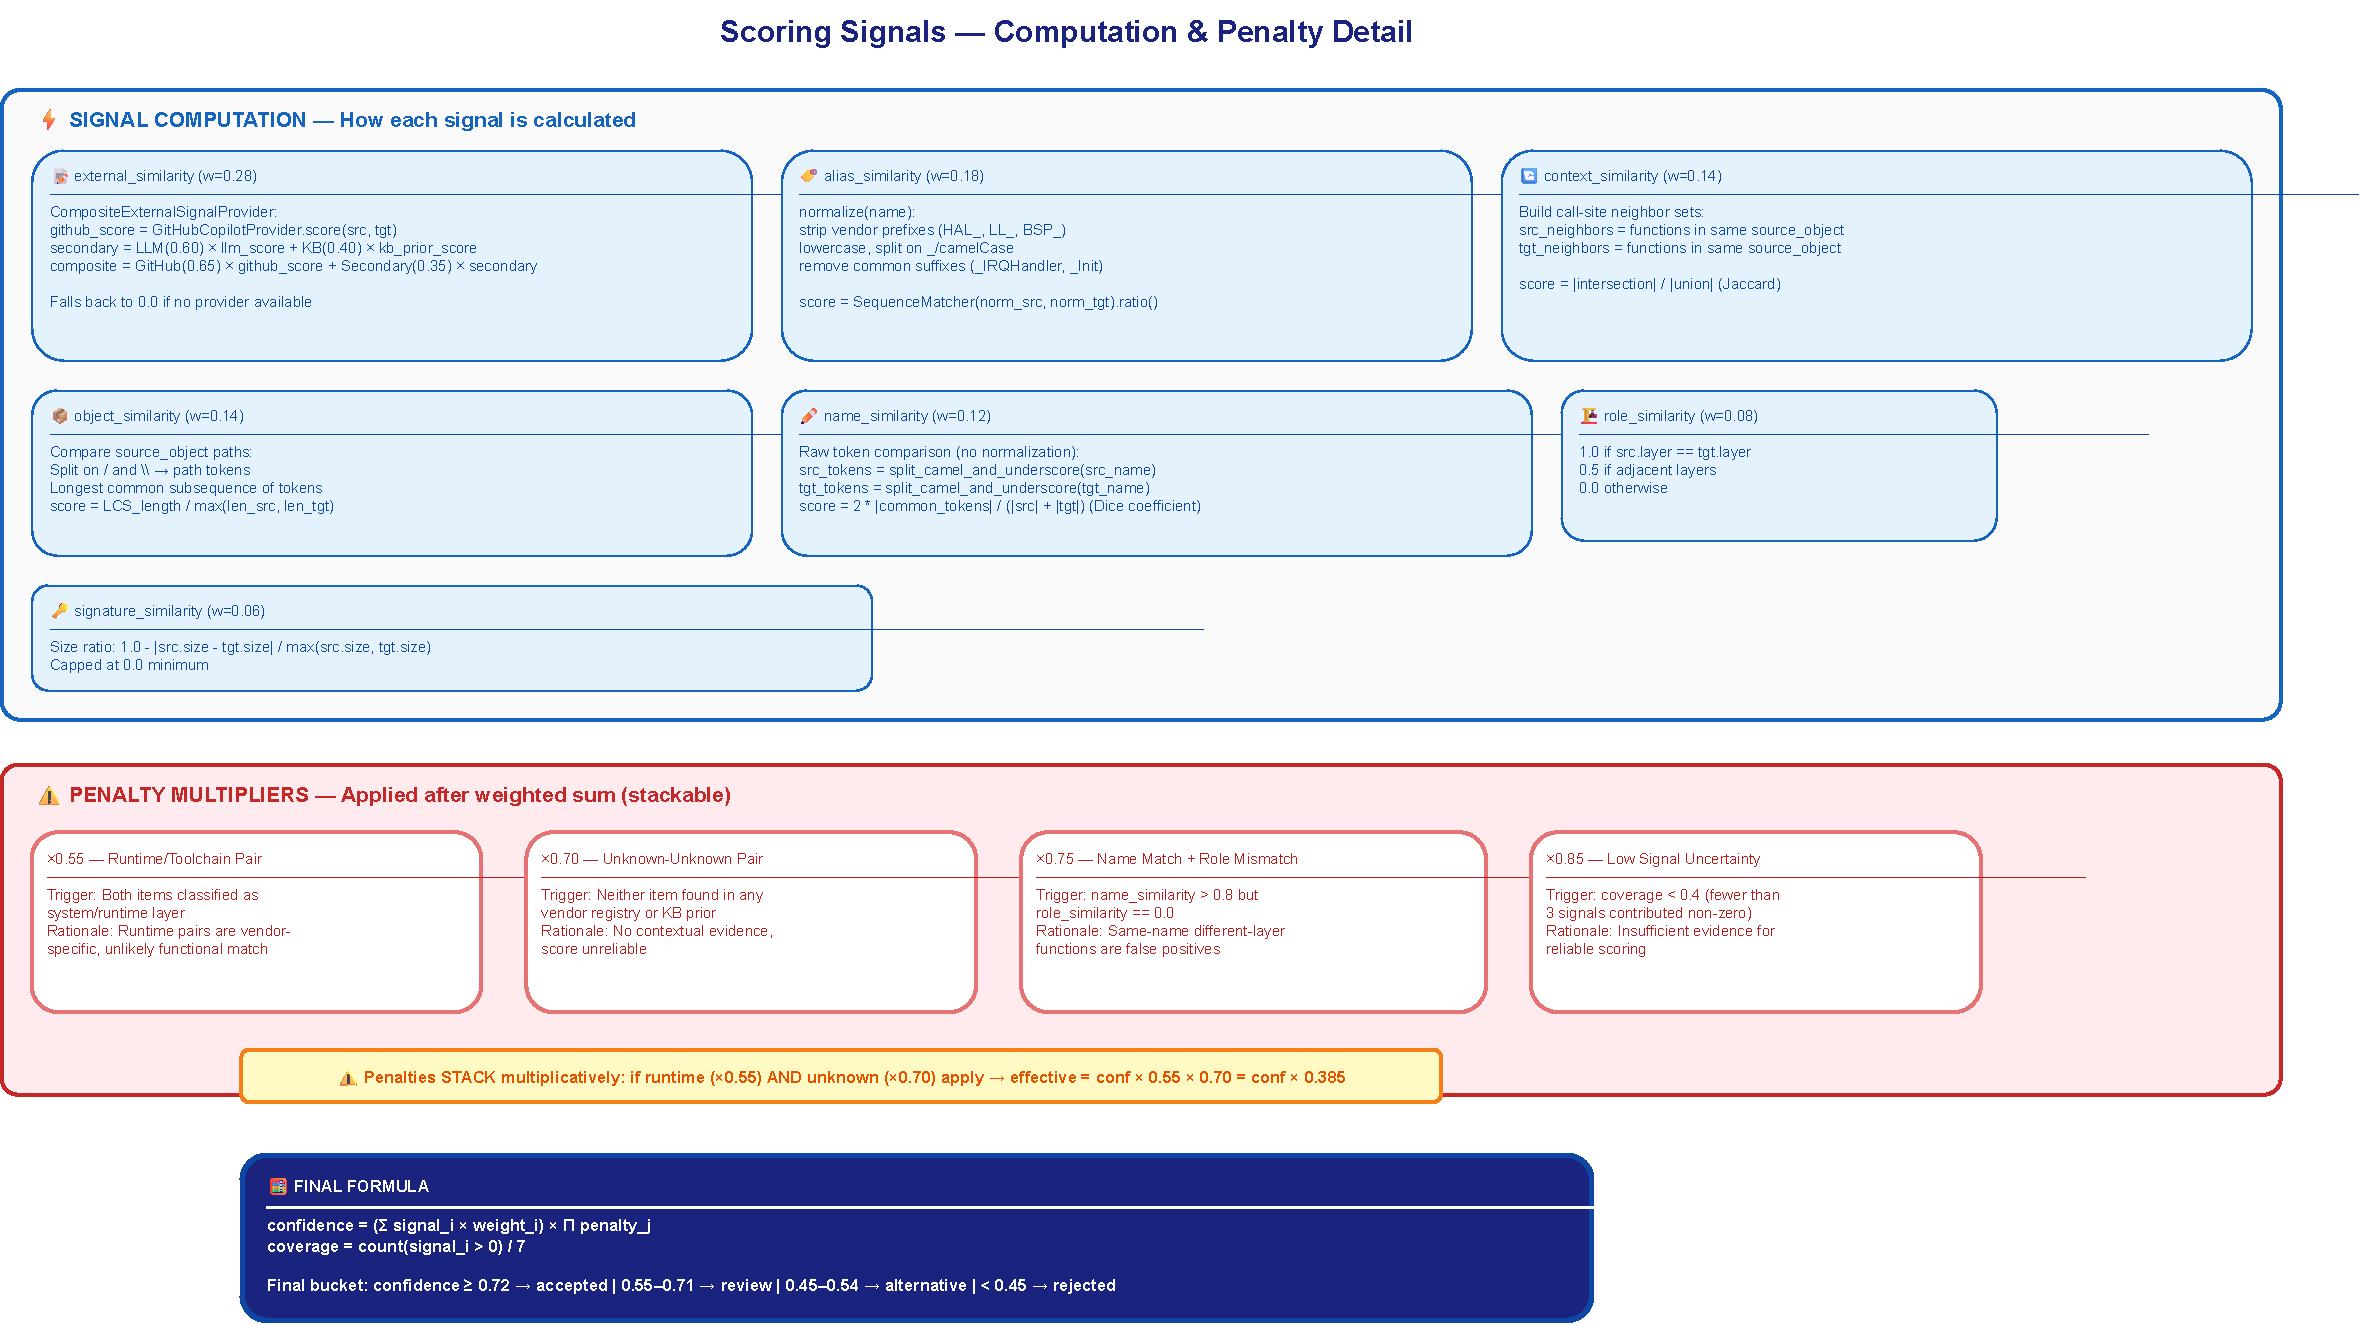
\includegraphics[width=\textwidth]{Figures/footprint-tool/scoring-signals.pdf}
\caption{Detailed signal computation and penalty system. Seven evidence signals are computed
for each candidate pair; penalties for size mismatch and layer conflict reduce the composite
score before the acceptance threshold is applied.}
\label{fig:tool-scoring-signals}
\end{figure}

The resulting confidence drives a transparent acceptance policy. A correspondence is accepted
automatically once its confidence reaches $0.72$, queued for manual review above $0.55$, kept
as a weaker alternative above $0.45$, and an unmatched symbol is retained on its own only above
$0.80$. The engine also records the cardinality of each match --- one-to-one, one-to-many, or
many-to-one --- which matters because vendors routinely split or merge functionality
differently, and a one-to-many match is itself a finding about how the two stacks are
structured. Every decision, with its per-signal breakdown, is written to the mapping
diagnostics so that a reviewer can see exactly why two symbols were paired.
Figure~\ref{fig:tool-candidate-ranking} illustrates the complete flow from candidate
generation through pruning, scoring, and threshold-based bucketing.

\begin{figure}[H]
\centering
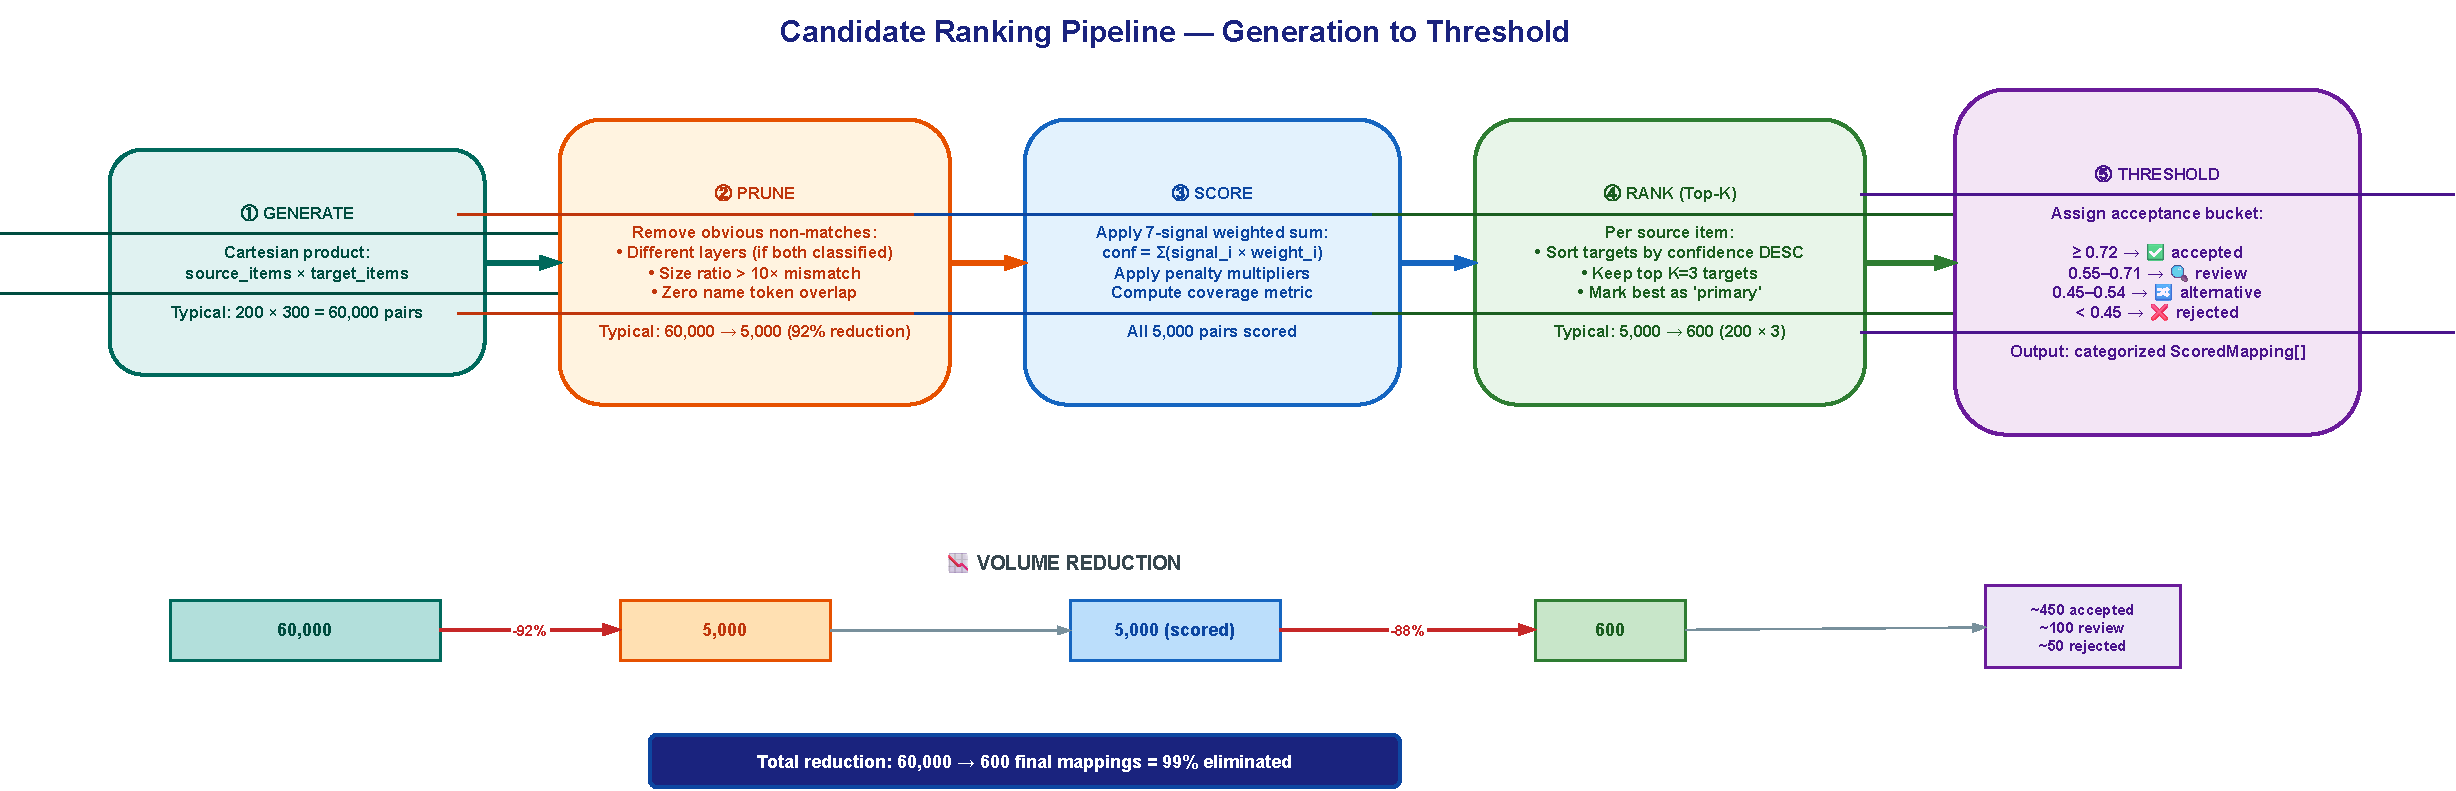
\includegraphics[width=\textwidth]{Figures/footprint-tool/candidate-ranking.pdf}
\caption{Candidate generation, ranking, and threshold flow. The Cartesian product of source
and target items is pruned by fast rejection filters, scored on all signals, and bucketed
into accepted, review, alternative, and unmatched categories by confidence thresholds.}
\label{fig:tool-candidate-ranking}
\end{figure}

\subsection{Optional AI assistance}
\label{sec:tool-ai}

The tool is best described as a deterministic core with \emph{optional} language-model
assistance, not as an "AI tool" in the sense of one that cannot work without a model. Every
language-model feature is opt-in and disabled by default, and the engine produces a complete,
reproducible result with all of them switched off. When they are enabled, they act in three
bounded ways. First, a large language model (LLM) can supply one additional
similarity signal during mapping; as Figure~\ref{fig:tool-weights} makes explicit, that signal
is weighted and capped so it can move a candidate's confidence by at most twelve percent, and
the run stays within a fixed call budget. Second, a "confident pass" may confirm or reject
borderline matches, and an advisor may suggest where STM32 firmware could be tightened.
Third, the desktop interface offers a chat assistant for exploring a comparison in natural
language.

These features can be served by several interchangeable back-ends, listed in
Table~\ref{tab:tool-ai}, selected automatically in a fixed order or pinned explicitly. They
range from a hosted GitHub Copilot endpoint~\cite{github-copilot} to a fully offline Ollama
server~\cite{ollama}, so the assistance can run without any data leaving the machine. If a
back-end is unavailable or returns something unusable, the tool degrades gracefully to its
deterministic output rather than failing. Figure~\ref{fig:tool-ai-integration} shows the
provider abstraction and the auto-detection fallback chain.

\begin{figure}[H]
\centering
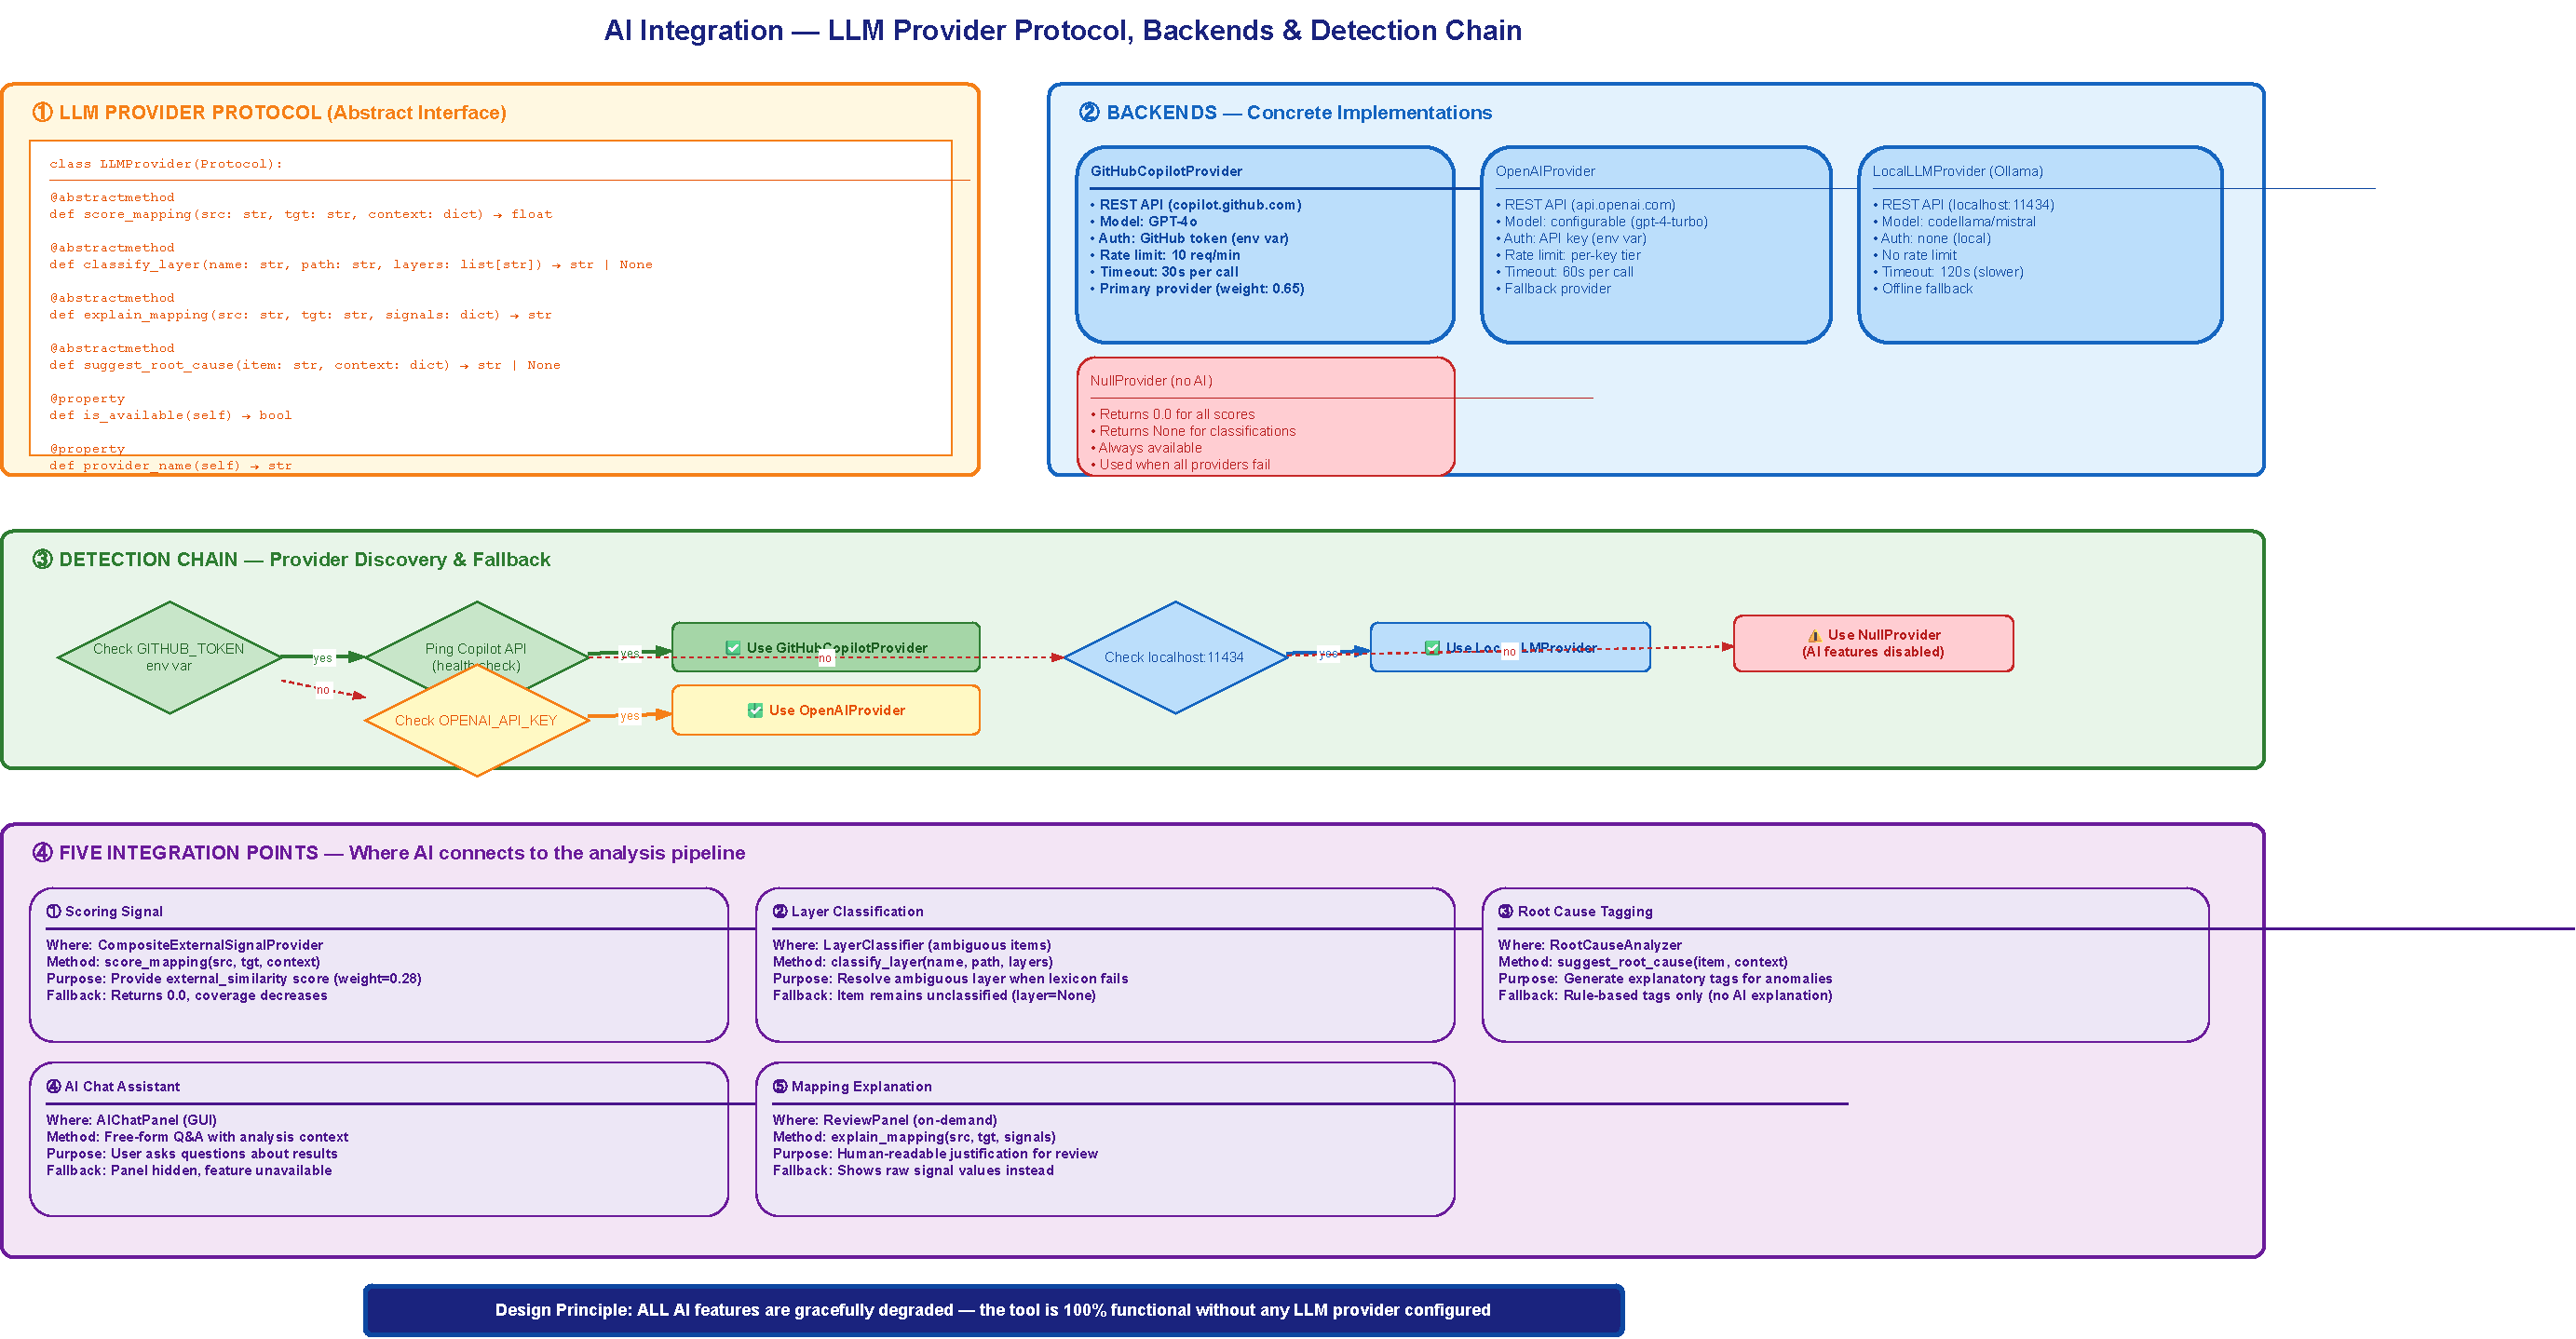
\includegraphics[width=\textwidth]{Figures/footprint-tool/ai-integration.pdf}
\caption{AI integration flow. A common protocol abstracts all back-ends; an auto-detection
chain probes them in priority order (Copilot, OpenAI, Ollama) and falls back gracefully to
purely deterministic operation if none is available.}
\label{fig:tool-ai-integration}
\end{figure}

\begin{table}[H]
\centering
\caption{Optional language-model back-ends. All are disabled by default; the tool runs fully
without them.}
\label{tab:tool-ai}
\begin{tabularx}{\textwidth}{l l X}
\toprule
\textbf{Back-end} & \textbf{Default model} & \textbf{Selection / requirement} \\
\midrule
GitHub Copilot \cite{github-copilot} & Claude (Anthropic) \cite{anthropic} & OAuth device flow; first in the auto-detect order. \\
OpenAI \cite{openai-api} & GPT-4o & \texttt{OPENAI\_API\_KEY} environment variable. \\
Ollama \cite{ollama} & Llama 3.1 (8B) & Local server; fully offline. \\
GitHub Models \cite{github-models} & gpt-4.1-mini & Default for the narrative assistant. \\
\bottomrule
\end{tabularx}
\end{table}

\subsection{Persistence and learning}
\label{sec:tool-persistence}

All state lives in local SQLite databases: the vendor registry, the store of confirmed
correspondences, a cache of assistant responses, and a history of runs. A manual confirmation
made during review can be replayed on later runs, so the tool improves as it is used on a given
vendor pair. We treat this learning, together with the web-ingestion and run-history features,
as useful but experimental, and none of it is on the critical path of a comparison.

\subsection{Cross-vendor equivalence database}
\label{sec:tool-equivalence}

A critical addition to the scoring engine is the \emph{cross-vendor equivalence database},
which encodes deterministic knowledge about which modules and functions serve the same
peripheral function across vendor SDKs. When two symbols are confirmed equivalents by this
database, their confidence is boosted to the high-confidence threshold regardless of naming
differences.

The database covers twenty-five peripheral groups (GPIO, UART, SPI, I\textsuperscript{2}C,
Timer, Clock, Power, DMA, USB Device, USB Host, Flash, ADC, DAC, CAN, Ethernet, RTC,
Watchdog, CRC, RNG, I\textsuperscript{2}S, Pin Mux, Interrupt, Cortex core, BSP/Board,
System Init, Startup, and PWM) with token-pattern entries for six vendors: STM32, NXP,
Renesas, TI, GigaDevice, and Infineon. It also encodes sixteen action-verb equivalence
classes (init/deinit, start/stop, transmit/receive, set/get, reset, callback, register/
unregister, lock/unlock, suspend/resume), so that \texttt{HAL\_GPIO\_Init} and
\texttt{GPIO\_Setup} are recognised as serving the same role.

The database is designed as an offline, provenance-tracked artefact: an equivalence miner
extracts entries from pinned vendor SDK repositories (resolved to a specific commit SHA for
reproducibility), records provenance for every entry, and produces a content-hashed mining
manifest. This ensures that the equivalence knowledge used in any given run is auditable
and frozen --- it cannot drift silently between executions.

\subsection{Source-code signal provider}
\label{sec:tool-source-code}

When both source and target IAR EWARM project directories are available, an optional
source-code signal provider enriches the mapping with three additional signals derived from
the actual C source files: function signature similarity (parameter count and return-type
patterns), call-graph structural similarity (shared callee patterns), and include-graph
co-location (functions in files with similar \texttt{\#include} dependencies). This
provider operates as an external-signal plug-in to the scoring engine and is disabled by
default; when enabled, it provides a richer correspondence basis for firmware that is
available locally, without requiring any network access or language model.

\subsection{Firmware quality metrics and grading}
\label{sec:tool-quality}

Beyond comparing two builds, the tool computes firmware quality metrics for the source
(STM32) firmware independently: total flash and RAM, module and function counts, average
and maximum module size, layer-balance score, modularity score, code density, HAL
abstraction ratio, middleware ratio, application ratio, large-module count, dead-weight
estimate, optimisation potential, and an overall quality grade (A through~F). These metrics
appear in the PDF report and help the technical marketing team assess not just how STM32
compares to a competitor, but how well the STM32 firmware itself is structured.

\subsection{Run manifest and reproducibility}
\label{sec:tool-manifest}

Every benchmark run emits a \emph{run manifest} that captures the tool version, the
deterministic mode (strict or assisted), the schema version, input file checksums, and a
hash of the equivalence database state at the time of execution. This manifest allows any
run to be proven reproducible: given the same inputs, configuration, and frozen knowledge
state, the tool must produce byte-for-byte identical logical output. The deterministic
hardening specification formalises this guarantee by requiring stable sort tie-breaks,
rounded floating-point scores, and canonical export ordering across all stages.

\section{Integration into the benchmark workflow}
\label{sec:tool-integration}

The tool occupies a precise place in our method. Once a software stack has been built for an
STM32 board and for the competing vendor's board under identical scenarios, each build's IAR
linker map is fed to the tool as the source and the target. Its per-layer and global footprint
figures, its verdict, and its root-cause breakdown are exactly the numbers the per-vendor
benchmarking chapters of this report quote when they weigh ST's flash and RAM cost against a
competitor's for a given stack. In other words, the footprint comparisons reported later are not
assembled by hand: they are produced, with an auditable trail, by the tool described here, which
is why we document it before presenting any results that depend on it.

\section{Usage and outputs}
\label{sec:tool-usage}

% TODO(screenshot): Replace placeholder with actual GUI screenshot
\begin{figure}[H]
\centering
\fbox{\parbox{0.9\textwidth}{\centering\vspace{4cm}\textbf{[PLACEHOLDER --- GUI screenshot]}\\Capture the MCU Workflow Studio desktop interface showing a completed\\benchmark comparison (main window with charts and layer breakdown).\vspace{4cm}}}
\caption{MCU Workflow Studio desktop interface showing a USB HID footprint comparison between STM32 and a competitor.}
\label{fig:tool-gui}
\end{figure}

A comparison can be driven either from the desktop interface or, for reproducible and scriptable
runs, from the command line. A typical invocation names the two maps and their vendors and points
at an output directory, as in Listing~\ref{lst:tool-cli}.

\lstset{style=mystyle}
\begin{lstlisting}[language=bash, caption={Command-line invocation of a footprint benchmark.}, label={lst:tool-cli}]
mcu-workflow-cli benchmark \
  --source stm32usbhidclassproject.map --source-vendor stm32 \
  --target nxpusbhidclassproject.map   --target-vendor nxp \
  --out results/
\end{lstlisting}

The run leaves behind the artefacts of Table~\ref{tab:tool-io}: a results workbook with the
per-layer and global comparison, scoped CSV/JSON exports, a prioritised review queue of the
matches that warrant a human look, the full mapping diagnostics, and --- on request --- an
eight-page PDF report with an executive summary, source-versus-target charts, an
architecture-and-module breakdown, a gap analysis, and recommendations. The samples we used to
develop and validate the tool are themselves a representative comparison: a USB human interface device (HID)
class project built for an STM32U575 board against the equivalent project built for an NXP
MCXN947 board~\cite{nxp-mcuxpresso}, both compiled with the same IAR toolchain so that only the
vendor software stacks differ.

% TODO(screenshot): Replace placeholder with actual Excel workbook screenshot
\begin{figure}[H]
\centering
\fbox{\parbox{0.9\textwidth}{\centering\vspace{3cm}\textbf{[PLACEHOLDER --- Results workbook screenshot]}\\Capture a screenshot of \texttt{benchmark\_results.xlsx} open in Excel, showing\\the per-layer comparison sheet with ROM/RAM columns.\vspace{3cm}}}
\caption{Sample output: the results workbook showing per-layer and global footprint comparison.}
\label{fig:tool-results-xlsx}
\end{figure}

% TODO(screenshot): Replace placeholder with actual PDF report page
\begin{figure}[H]
\centering
\fbox{\parbox{0.9\textwidth}{\centering\vspace{3cm}\textbf{[PLACEHOLDER --- PDF report screenshot]}\\Capture the first page (executive summary) of the optional PDF report\\generated by the tool, showing the verdict chart.\vspace{3cm}}}
\caption{First page of the optional PDF report: executive summary with source-vs-target charts.}
\label{fig:tool-pdf-report}
\end{figure}

\section{Engineering value and limitations}
\label{sec:tool-value}

The value of the tool is that it turns a slow, subjective, once-off comparison into a fast,
explainable, and repeatable one. A footprint benchmark that previously took an afternoon of
careful map-reading now runs in seconds and produces the same answer every time, with a
documented reason behind every symbol correspondence and a clear attribution of where each
kilobyte of difference originates. The run manifest, the frozen equivalence database, and the
deterministic hardening guarantee that the same inputs always yield the same verdict ---
satisfying the reproducibility requirement of academic evaluation.

The twelve-signal scoring engine, backed by the cross-vendor equivalence database covering
twenty-five peripheral groups and sixteen action-verb classes, achieves high-confidence
mappings across six vendors without relying on language models. The firmware quality metrics
and grading system provide an independent structural assessment of the STM32 firmware, and
the multi-run history tracks how footprint evolves across SDK versions.

We are equally clear about what the tool does not do. It reads IAR EWARM linker maps; builds
produced by other toolchains are out of scope for now, and broadening the parser is the most
obvious avenue for future work. Its footprint figures are static, derived from the linked image
rather than from execution. The quality grades and optimisation-potential estimates that the
report produces are heuristic indications, not measured quantities, and we label them
accordingly wherever they appear. Finally, the language-model features, while useful, are
optional and still maturing; the trustworthy core of the tool is, and is meant to remain, fully
deterministic.

\section*{Conclusion}

We designed and built MCU Workflow Studio to remove the manual bottleneck in cross-vendor
footprint benchmarking and to make its results reproducible and explainable. Its deterministic
core parses two IAR linker maps, classifies every symbol into an architectural layer, maps
STM32 symbols to their competitor counterparts using a twelve-signal scoring engine backed by a
cross-vendor equivalence database, and reports per-layer and global flash and RAM differences
with a clear root cause. The run manifest guarantees reproducibility; the firmware quality
metrics provide an independent structural assessment; and the optional, strictly bounded
language-model assistance enriches the mapping without ever sitting on the critical path. The
chapters that follow rely on this tool for the footprint figures they report, which is why we
have presented it first, as a contribution in its own right.
